\section{Duality? What is it?}

\noindent
In the previous parts we tried to persuade the reader that linear programming is a powerful and flexible
tool for solving optimization problems, and, in particular, for the design of approximation algorithms. 
Now we shall introduce another crucial feature of linear programs, called {\em duality},
that is also often employed in the design 
of algorithms. Let us imagine that Robert wants to find the minimum of a function
$$f(x_1,x_2,x_3):=10x_1+3x_2+5x_3$$ 
over the values $x_1, x_2, x_3$ that satisfy
\begin{eqnarray}
\label{LP_001}6x_1 + \phantom{2}x_2 - \phantom{3}x_3&\ge&2\\
\label{LP_002}2x_1 + 2x_2 + 6x_3&\ge&8\\
6x_1 + 3x_2 + 5x_3&=&30\nonumber\\
x_1,x_2,x_3&\ge&0\nonumber
\end{eqnarray}
Angela immediately sees that this is a linear program, and easily finds the minimum. The question is, 
how she can make Robert, ho knows nothing about linear programming, believe her. For an upper bound,
she could present him with a {\em witness}, i.e. a particular solution (e.g. a vector  $x_1=2$, $x_2=6$, $x_3=0$)
that makes him believe that the minimum is at most some value (e.g. 38, in this case). But what can Angela
do to find a witness of a lower bound? She may try the following argument: {\em ''Look at the line 
(\ref{LP_001}). No matter how you choose the three non-negative numbers $x_1, x_2, x_3$, it will always hold
$6x_1\le10x_1$, $x_2\le3x_2$, and $-x_3\le5x_3$, so $6x_1+x_2-x_3\le f(x_1,x_2,x_3)$. However, according
to  (\ref{LP_001}) for any feasible solution it holds  $6x_1+x_2-x3\ge2$, and so for any feasible solution
(in particular, for the minimum) it holds $f(x_1,x_2,x_3)\ge 2$''}. Robert will accept this argument, and
she can continue e.g. arguing that if the lines (\ref{LP_001}) and  (\ref{LP_002})
are added together, the same argument can be used. Also, each line can be multiplied by some number
(it must be a non-negative number for lines (\ref{LP_001}) and (\ref{LP_002})) and then add them together:
if it holds that the resulting linear combination of the left-hand sides of the constraints is component-wise
smaller than the utility function $f$, the corresponding linear combination of the right-hand sides gives
a lower bound on the minimum. When Robert is willing to accept all these arguments, Angela, in order to give
the best possible lower bound, solves a linear program: to find a maximum of the function 
$$g(y_1,y_2,y_3):=2 y_1+8 y_2+30 y_3$$
among those values  $y_1, y_2, y_3$ that satisfy
\begin{eqnarray*}
6y_1 + 2y_2 + 6y_3 &\le& 10\\
y_1 + 2y_2 + 3y_3 &\le& 3\\
-y_1 + 6y_2 + 5y_3 &\le& 5\\
y_1,y_2 &\ge& 0
\end{eqnarray*}
In this case, on one hand there is a witness $x_1=0$, $x_2=5$, $x_3=3$ asserting that the minimum of $f$ is at 
most 30, on the other hand, there is witness  $y_1=y_2=0$, $y_3=1$ showing that minimum is at least 30.
Was Angela just lucky that she managed to find witnesses for the exact optimum?

\noindent
Now let us have a closer look at what is happening in the general case. Consider a following linear program that we 
shall call {\em primary}:

$$
\begin{array}{rrrrrcl}
  {\rm minimize}     & c_1x_1     & + c_2x_2       & + \cdots  & +c_nx_n  \\
  {\rm subject\ to} & a_{1,1}x_1 & + a_{1,2}x_2   & + \cdots  & +a_{1,n}x_n  & \ge & b_1 \\
                          & a_{2,1}x_1 & + a_{2,2}x_2   & + \cdots  & +a_{2,n}x_n  & \ge & b_2 \\
                          &   \vdots   &   \vdots       &   \ddots   &  \vdots      &  \vdots & \vdots\\ 
                          & a_{m,1}x_1 & + a_{m,2}x_2   & + \cdots  & +a_{m,n}x_n  & \ge & b_m \\
                          &\multicolumn{4}{r}{x_1,\ldots,x_n}&\ge&0
\end{array}
$$
or, using a more concise notation
$$ (P): \min_{\bm{x}\in\R^n}\left\{ \bm{c}\tr\bm{x} \mid A\bm{x}\ge\bm{b},\;\bm{x}\ge\bm{0}\right\}.$$

\noindent
We seek a  lower bound on the minimum of $(P)$ as a suitable linear combination of the constraints:
the $j$-th constraint is multiplied on both sides by some coefficient $y_j\ge0$, and the results are 
added together. We want to find the coefficients $y_j$ such that the left-hand side is component-wise
smaller than
the utility function

$$ \sum\limits_{i=1}^nc_ix_i\ge \sum\limits_{j=1}^m y_j 
\left(a_{j,1}x_1 + a_{j,2}x_2 + \cdots + a_{j,n}x_n\right) \ge  \sum\limits_{j=1}^my_j\cdot b_j. $$

Since all $x_i\ge0$, if $c_i\ge\sum_{k=1}^my_ja_{j,i}$, the first inequality holds.So the best lower
bound we can obtain from this approach is the solution of {\em dual} linear program

$$
\begin{array}{rrrrrcl}
  {\rm maximize}     & b_1y_1     & + b_2y_2       & + \cdots  & +b_my_m  \\
  {\rm subject\ to} & a_{1,1}y_1 & + a_{2,1}y_2   & + \cdots  & +a_{m,1}y_m  & \le & c_1 \\
                          & a_{1,2}y_1 & + a_{2,2}y_2   & + \cdots  & +a_{m,2}y_m  & \le & c_2 \\
                          &   \vdots   &   \vdots       &   \ddots   &  \vdots      &  \vdots & \vdots\\ 
                          & a_{1,n}y_1 & + a_{2,n}y_2   & + \cdots  & +a_{m,n}y_n  & \le & c_n \\
                          &\multicolumn{4}{r}{y_1,\ldots,x_m}&\ge&0
\end{array}
$$
or, using a more concise notation
$$ (D): \max_{\bm{y}\in\R^m}\left\{ \bm{b}\tr\bm{y} \mid A\tr\bm{y}\le\bm{c},\;\bm{y}\ge\bm{0}\right\}.$$

\noindent
Our musings so far are summarized in the following theorem, known as a {\em weak duality theorem}: 

\begin{veta}\label{thm:weakduality}
  If \bm{x} is an arbitrary feasible solution of the primal program  $(P)$, and
  \bm{y} is an arbitrary feasible solution of the dual program $(D)$, it holds
$$\bm{c}\tr\bm{x}\ge\bm{b}\tr\bm{y}$$
\end{veta}
\begin{dokaz}
\begin{equation}
\label{eq:weakduality}
\bm{c}\tr\bm{x}\ge\left(A\tr\bm{y}\right)\tr\bm{x}=\bm{y}\tr A\bm{x}\ge\bm{y}\tr\bm{b}
\end{equation}
The first inequality follows from the constraints of the dual program: since \bm{y} is
a feasible solution of the dual program, it holds $\bm{c}\ge A\tr\bm{y}$.
Similarly, the second inequality follows from the constraints of the primal program: since \bm{x}
is a feasible solution of the primal program, it holds $A\bm{x}\ge\bm{b}$.
\end{dokaz}

\noindent Theorem~\ref{thm:weakduality} should come as no surprise to the reader, since it only states
how we created the dual program: all feasible solutions of $(D)$ are lower bounds on the minimum
of $(P)$. The curious fact in our case was that the values of the optimal solutions of primal and dual
program were equal. In the next part we show that this was not a coincidence. Before we do so, however,
let us note some observations about the construction of the dual program. In the introductory example,
the goal of the primal program was minimization, and we were seeking the best possible lower bound on the minimum, 
so the goal of the dual program was maximization. However, all our reasoning was symmetrical with respect
to this, so we could start from a maximization program, and seek, using the same method, an upper bound on the
maximum; we would get a minimization dual program. The reader easily verifies that the primal and dual 
programs are completely symmetrical: if we started from the program $(D)$ as primal, we would get a dual 
program $(P)$. Hence, a dual program of a dual program is the primal program.

\noindent 
Finally, let us observe the form of the constraints. In the introductory example the primal program 
had constraints in the form of both inequalities ($\ge$), and equality. In the first case, the corresponding
multipliers $y_i$ had to be non-negative, in the case of equality, the multiplier could be an arbitrary real 
number. At the same time, all the variables $x_i$
in the primal program were constrained to be non-negative, so it was sufficient to have the constraints in the
dual program in the form of inequalities. What would happen if some variable, say, $x_1$ could be also negative?
In the same way as when we defined the normal form of a linear program we could replace $x_1=z_1-z_2$
for two fresh variables $z_1,z_2\ge0$, obtaining a primal program
minimize
$$f(z_1,z_2,x_2,x_3):=10z_1-10z_2+3x_2+5x_3$$ 
over values $z_1, z_2, x_2, x_3$ satisfying
\begin{eqnarray}
\label{LP_001a}6z_1 -6z_2 + \phantom{2}x_2 - \phantom{3}x_3&\ge&2\\
\label{LP_002a}2z_1 -2z_2 + 2x_2 + 6x_3&\ge&8\\
              6z_1 -6z_2 + 3x_2 + 5x_3&=&30\nonumber\\
z_1,z_2,x_2,x_3&\ge&0\nonumber
\end{eqnarray}
The corresponding dual program would ask to minimize the function
$$g(y_1,y_2,y_3):=2 y_1+8 y_2+30 y_3$$
over values $y_1, y_2, y_3$ satisfying
\begin{eqnarray*}
6y_1 + 2y_2 + 6y_3 &\le& 10\\
-6y_1 - 2y_2 - 6y_3 &\le& -10\\
y_1 + 2y_2 + 3y_3 &\le& 3\\
-y_1 + 6y_2 + 5y_3 &\le& 5\\
y_1,y_2 &\ge& 0
\end{eqnarray*}
where the first two inequalities can be combined into one equation  $6y_1+2y_2+6y_3=10$.
Summarizing, the dual program is constructed according to the following rules:

\vskip 2ex
\centerline{\begin{tabular}{|ll|ll|}\hline
\multicolumn{2}{|c|}{\rule{0mm}{3ex}{\bf primal program}}&\multicolumn{2}{|c|}{{\bf dual rpgram}}\\[1mm]\hline
\rule{0mm}{3ex}minimize & $\bm{c}^T\bm{x}$ & maximize & $\bm{b}^T\bm{y}$\\
\rule{0mm}{3ex}$i$-th constraint & $\displaystyle\sum_{j=1}^na_{ij}x_j=b_i$ &
$i$-th variable & $y_i\in{\mathbb R}$\\
\rule{0mm}{3ex}$i$-th constraint & $\displaystyle\sum_{j=1}^na_{ij}x_j\ge b_i$ &
$i$-th variable & $y_i\ge 0$\\
$j$-th variable & $x_j\in{\mathbb R}$&
\rule{0mm}{3ex}$j$-th constraint & $\displaystyle\sum_{i=1}^ma_{ij}y_i=c_j$\\
$j$-th variable & $x_j\ge0$&
\rule{0mm}{3ex}$j$-th constraint & $\displaystyle\sum_{i=1}^ma_{ij}y_i\le c_j$\\
\hline
\end{tabular}}
\vskip 4ex

\IGNORE{Dan Spielman}

\noindent
Before proceeding towards
our goal to show that the common optimum of our primal and dual programs was not a coincidence,
let us make a small trip into the land of algebraic topology.


\vspace*{-4ex}
\noindent
\colorlet{shadecolor}{Aquamarine!9}
\begin{shaded}
\subsection*{A short visit to convex hulls}

\noindent
The reader probably have already encountered the convex hull in two dimensions: for a given set of
points in the plane, the convex hull is the smallest polygon that contains all of them. 
\noindent
\begin{minipage}[t]{3.5cm}
  \vspace{0pt}
  \begin{myfig}{\textwidth}{svg/ko2d}
  \end{myfig}
\end{minipage}\hspace*{1cm}\begin{minipage}[t]{\textwidth-4.5cm}
  \vspace{0pt}
\noindent
If we imagine the points as poles, if we wrap a rope around them then the poles touched by the rope form
the convex hull. This intuition can work quite good also in three dimensions, where the convex hull is
obtained by wrapping a set of points by a sheet of paper. Having $n$-dimensional points and a sheet of
$n-1$-dimensional paper is somewhat more complicated to visualize; not all the properties that we 
take as granted in 2 dimensions hold also in the $n$-dimensional case. That's why we 
\end{minipage}

\vspace*{-8mm}
\noindent
need to be extra
suspicious about arguments like {\em ''it is obvious that...''}, and we need a more formal approach.
Recall that a convex body $\cal T$ is a set of points such that for any two points 
$\bm{x},\bm{y}\in{\cal T}$ the whole connecting line is in $\cal T$, i.e. all the points of the form 
$t\bm{x}+(1-t)\bm{y}$ for $0\le t\le 1$. Let us define the convex hull as follows:

\begin{dfn}
The convex hull of $n$ points $\bm{a}_1,\ldots,\bm{a}_n$ 
is the intersection of all convex bodies that contain the points $\bm{a}_1,\ldots,\bm{a}_n$.
\end{dfn}

\noindent
There are uncountably many convex bodies containing a given set of points, but their intersection is
well defined, so we don't care. Moreover, intersection of an arbitrary number of convex bodies is again convex,
so our definition is nice in the respect that the convex hull is, as one would expect, convex. The following
characterization comes in handy:

\begin{lema}
  \label{lm:KO:1}
  The convex hull of a set of $n$ points 
$\bm{a}_1,\ldots,\bm{a}_n$ 
is formed by the points that are {\em convex combinations} of the points $\bm{a}_1,\ldots,\bm{a}_n$, i.e.
are of the form  $z_1\bm{a_1}+\cdots+z_n\bm{a}_n$,
where
 \hbox{$z_1,\ldots,z_n\in\R^+$} a $z_1+\cdots+z_n=1$.  
\end{lema}


\begin{dokaz}
  Denote by $K$ the set of all convex combinations of the points $\bm{a_1},\ldots,\bm{a_n}$.
  It is easy to verify that $K$ is a convex body: for convex combinations  $\sum z_i\bm{a_i}$
  and  $\sum z'_i\bm{a_i}$ is also $t\sum z_i\bm{a_i} + (1-t)\sum z'_i\bm{a_i} = \sum (tz_i+(1-t)z'_i)\bm{a_i}$
  a convex combination, and so belongs to $K$. Since $K$ is a convex body containing the points
  $\bm{a_1},\ldots,\bm{a_n}$,
  by definition $K$ contains their convex hull. To prove the lemma it suffices to show that every convex combination 
  is contained in the convex hull.

  \noindent
  We prove it by induction on the number of points $n$. For $n=1$ it follows directly from the definition of 
  convex hull, for $n=2$ the convex combinations are  $z_1\bm{a_1}+(1-z_1)\bm{a_2}$ and these, due to convexity,
  are in any convex body containing $\bm{a_1}$ and  $\bm{a_2}$ (and so they are contained in the intersection
  of them). Now let $n\ge 3$, and consider a convex combination  $\bm{x}=\sum z_ia_i$. If $z_n=1$, $\bm{x}=\bm{a_n}$
  and \bm{x} it is in the convex hull by definition. So let $z_n<1$, and denote  $z'_i:=\frac{z_i}{1-z_n}$.
  Considering the point $\bm{x'}=\sum z'_i\bm{a_i}$, we see it is a convex combination of points 
  $\bm{a_1},\ldots,\bm{a_{n-1}}$, and by the induction hypothesis any convex body containing 
  $\bm{a_1},\ldots,\bm{a_{n-1}}$ contains also \bm{x'}. At the same time,  $\bm{x}=(1-z_n)\bm{x'}+z_n\bm{a_n}$
  implying that any convex body containing both \bm{x'} and $\bm{a_n}$ contains also \bm{x}.
\end{dokaz}

%\vspace*{-3ex}
\noindent
\begin{minipage}[t]{6cm}
  \vspace{0pt}
\begin{center}
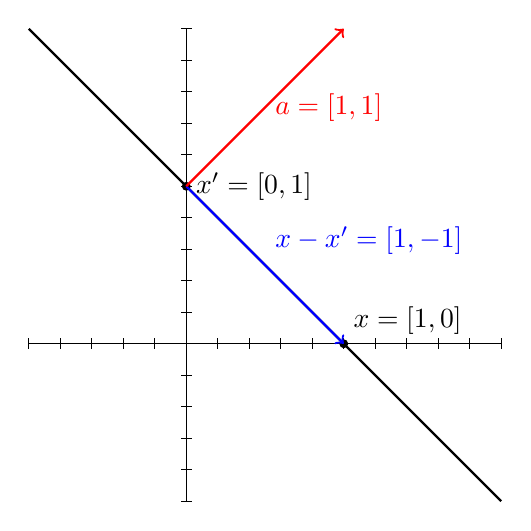
\begin{tikzpicture}[scale=2]
  %axis
  \draw (-1,0) -- coordinate (x axis mid) (2,0);
  \draw (0,-1) -- coordinate (y axis mid) (0,2);
  %ticks
  \foreach \x in {-1,-0.8,...,2}
    \draw (\x,1pt) -- (\x,-1pt);
  \foreach \y in {-1,-0.8,...,2}
  \draw (1pt,\y) -- (-1pt,\y);


  \draw[thick] (-1,2) -- (2,-1); 

  \fill (1,0) circle (.8pt) node [anchor=south west] {$x=[1,0]$};
  \fill (0,1) circle (.8pt) node [anchor=west] {$x'=[0,1]$};

  \draw[thick,->,blue] (0,1) -- node [anchor = south west] {$x-x'=[1,-1]$}  (1,0);
       
  \draw[thick,->,red] (0,1) -- node [anchor=west] {$a=[1,1]$} (1,2);

\end{tikzpicture}

\end{center}

\end{minipage}\hspace*{1cm}\begin{minipage}[t]{\textwidth-7cm}
  \vspace{0pt}
  Recall that in an $n$-dimensional space, a hyperplane $\cal H$ is a set of points \bm{x} satisfying
  an inequality $a_1x_1+\cdots+a_mx_m=1$ (the number one on the right hand side is almost without loss of
  generality: any hyperplane that does not contain the point  $[0,\ldots,0]$ can be normalized to this form).
  If we use the notation  $\pair{\cdot}{\cdot}$ for the scalar product, $\cal H$ is defined by 
   $\pair{\bm{x}}{\bm{a}}=1$. The points for which  $\pair{\bm{x}}{\bm{a}}<1$ are below the hyperplane,
   and points $\pair{\bm{x}}{\bm{a}}>1$ are above it. The vector \bm{a} is called a {\em normal } vector
   of $\cal H$ and for any two points \bm{x}, \bm{x'} from $\cal H$ it holds 
$$\pair{\bm{x}-\bm{x'}}{\bm{a}}=\sum_{i=1}^m(x_i-x'_i)a_i=\pair{\bm{x}}{\bm{a}}-\pair{\bm{x'}}{\bm{a}}=0.$$

\noindent
In two dimensions the hyperplane is a line; the one on the figure on the left is given by the equation
$x_1+x_2=1$.

\end{minipage}

\vskip 2mm
\noindent
Our discussion about convex hull concludes with the following observation that is completely obvious for two and 
three dimensions:

\begin{lema}
  \label{lm:KO:2}
  Consider points  $\bm{x},\bm{a_1},\ldots,\bm{a_n}$ in an $m$-dimensional space. 
  Let $K$ be the convex hull of 
  $\bm{a_1},\ldots,\bm{a_n}$. The it holds:
  \begin{itemize}
    \item 
      If \bm{x} is inside (i.e. $K$ contains \bm{x} with some small neighborhood) $K$, 
      then there is no hyperplane $\cal H$ 
      containing \bm{x} such that all points from $K$ are on one side
      (above or below) of $\cal H$.
    \item 
      If $\bm{x} \not\in K$,
      then there exists a hyperplane $\cal H$
      containing \bm{x} such that all points from $K$ are on one side
      (above or below) of $\cal H$.
  \end{itemize}
\end{lema}

\begin{dokaz}
  The first part is easy: let \bm{x} be inside $K$, and suppose there exists a hyperplane $\cal H$ such that
  all points from $K$ are one one side of $\cal H$. Since $\cal H$ contains \bm{x},
  there are two points in any close neighborhood of \bm{x} that lie on different sides of $\cal H$. 
  But \bm{x} is inside $K$, so there is some small neighborhood of \bm{x} contained in $K$.

\noindent
Now let us show the second part.
Consider a fixed point \bm{x}, and for all points $\bm{y}\in K$ consider the Euclidean distance 
$f(\bm{y}):=||\bm{y}-\bm{x}||$. Since $K$ is a compact set, and $f$ is a continuous function with positive codomain,
there is a point  $\bm{z}\in K$ where $f$ reaches minimum. Denote
  \begin{align*}
    \bm{t}&=\bm{x}-\bm{z} & \kappa&= \pair{\bm{t}}{\bm{x}}
  \end{align*}

\begin{minipage}[t]{4.5cm}
  \vspace{0pt}
  \begin{myfig}{\textwidth}{svg/CHa}
  \end{myfig}
\end{minipage}\hspace*{1cm}\begin{minipage}[t]{\textwidth-7cm}
  \vspace{0pt}
  Let$\cal H$ be the hyperplane consisting of points  \bm{y} for which $\pair{\bm{t}}{\bm{y}}=\kappa$.
  Clearly $\bm{x}\in{\cal H}$. It holds
  $$0\le\sum_{i=1}^m(x_i-z_i)^2=%\sum_{i=1}^mx_i^2-2x_iz_i+z_i^2=
  \bpair{x}{x}-2\bpair{x}{z}-\bpair{z}{z}$$
  and so
  \begin{align*}&\bpair{t}{z}=\pair{\bm{x}-\bm{z}}{\bm{z}}=\bpair{x}{z}-\bpair{z}{z}\le\\
                &\le\bpair{x}{x}-\bpair{x}{z}=\pair{\bm{x}-\bm{z}}{\bm{x}}=\bpair{t}{x}=\kappa
  \end{align*}
  \noindent
  Now it suffices to show that for all points $\bm{y}\in K$ it holds $\bpair{t}{y}\le\kappa$, and so
  they are on the same side of $\cal H$ as \bm{z}.
\end{minipage}

\noindent
Hence, let us consider $\bm{z}\in K$. 
Since \bm{z} minimizes the distance from  \bm{x}, and $K$ is a convex body, for all  $0\le\lambda\le1$ it holds
$||\bm{z}-\bm{x}||^2\le||(1-\lambda)\bm{z}+\lambda\bm{y}-\bm{x}||^2=
||(1-\lambda)(\bm{z}-\bm{x})+\lambda(\bm{y}-\bm{x})||^2$,
and from that after straightforward calculation
$0\le\lambda(\lambda-2)||\bm{z}-\bm{x}||^2+2\lambda(1-\lambda)\pair{\bm{z}-\bm{x}}{\bm{y}-\bm{x}}
+\lambda^2||\bm{y}-\bm{x}||^2
$.
Since $\lambda\ge0$, we have
$0\le(\lambda-2)||\bm{z}-\bm{x}||^2+2(1-\lambda)\pair{\bm{z}-\bm{x}}{\bm{y}-\bm{x}}
+\lambda||\bm{y}-\bm{x}||^2
$
and from that for the limit case  $\lambda\mapsto0$
we get $0\le\pair{\bm{z}-\bm{x}}{\bm{y}-\bm{x}}-||\bm{z}-\bm{x}||^2
=\pair{\bm{z}-\bm{x}}{\bm{y}-\bm{x}}-\pair{\bm{z}-\bm{x}}{\bm{z}-\bm{x}}
=\pair{\bm{z}-\bm{x}}{\bm{y}}-\pair{\bm{z}-\bm{x}}{\bm{z}}=\bpair{t}{z}-\bpair{t}{y}
$.
That's why
$\bpair{t}{y}\le\bpair{t}{z}\le\kappa$, what we wanted to prove.
\end{dokaz}

\end{shaded}

\noindent
Now let us get back to our goal -- to show that the same value of the primal and dual program we obtained
was not a coincidence. Let us consider the following example: for given $n$ points
 $\bm{a}_1,\ldots,\bm{a}_n$ from the
$m$-dimensional space
$\R^m$ (i.e. the point $\bm{a}_i$ has coordinates  $(a_{i1},a_{i2},\ldots,a_{im})$), and a vector 
$\bm{c}$, the goal is to find a largest possible number $\alpha\in\R^+$ such that  the point 
$\alpha\bm{c}$ is contained in the convex hull $K$ of the points  $\bm{a}_1,\ldots,\bm{a}_n$. 

\begin{minipage}[t]{3.2cm}
  \vspace{0pt}
  \begin{myfig}{\textwidth}{svg/dualityCHa}
  \end{myfig}
\end{minipage}\hspace*{1cm}\begin{minipage}[t]{\textwidth-5cm}
  \vspace{0pt}
  \vskip 2ex
\noindent 
Let us suppose, for the ease of exposition, that there is some solution, i.e. that the ray
generated by the vector $c$ hits $K$. From the convexity it follows that the intersection of $K$ and a line
is a line segment. The optimal solution is thus the point $\alpha\bm{c}$ where the ray leaves $K$. Following
Lemma~\ref{lm:KO:1}, the points of the convex hull can be expressed as a convex combination of the points
 $\bm{a}_1,\ldots,\bm{a}_n$,
 i.e. our unknown point $\alpha\bm{c}$ must be of the form $z_1\bm{a}_1+\cdots+z_n\bm{a}_n$
for some  $z_1,\ldots,z_n\ge0$ where  $\sum_{i=1}^nz_i=1$. 
Denoting  $y_j=\frac{z_j}{\alpha}$
for an arbitrary feasible point  $\alpha\bm{c}$ yields
\end{minipage}
\vspace*{-18mm}
  \begin{align*}
    y_j\ge&0 & \sum_{j=1}^ny_j=\frac{1}{\alpha} && \alpha\bm{c}=\alpha\sum_{j=1}^n\bm{a}_jy_j.
  \end{align*}
  To find a point that maximizes $\alpha$ means to find a point that minimizes $1/\alpha$.
  So we want to minimize the value  $\sum_{j=1}^ny_j$ over those $y_1,\ldots,y_n\ge 0$ for which
  $\sum_{j=1}^n\bm{a}_jy_j=\bm{c}$; just note that from given \bm{y}, \bm{z} and $\alpha$ can be reconstructed.
  Our task can be written as a linear program:
\begin{equation}
  \label{eq:dualCHa}
\begin{array}{rrrrrcl}
  {\rm minimize}     & y_1        & +\;y_2         & +\; \cdots  & +\;y_n   \\
  {\rm subject\ to} & a_{1,1}y_1 & +\;a_{2,1}y_2   & +\; \cdots  & +\;a_{n,1}y_n  & = & c_1 \\
            %              & a_{1,2}y_1 & +\;a_{2,2}y_2   & +\; \cdots  & +\;a_{n,2}y_n  & = & c_2 \\
                          &   \vdots   &   \vdots       &   \ddots   &  \vdots      &  \vdots & \vdots\\ 
                          & a_{1,m}y_1 & +\; a_{2,m}y_2   & +\; \cdots  & +\;a_{n,m}y_n  & = & c_m \\
                          &\multicolumn{4}{r}{y_1,\ldots,y_n}&\ge&0
\end{array}
\end{equation}

\noindent
or shorter
$$\text{(P)}\;\; \min_{\bm{y}\in\R^n}\left\{ \bm{1}\tr\bm{y} \mid A\tr\bm{y}=\bm{c},\;\bm{y}\ge\bm{0}\right\}, $$
where $A$ is an $n\times n$ matrix with rows formed by the coordinates of points  $\bm{a}_1,\ldots,\bm{a}_n$.
We apply our dualization recipe to the program (\ref{eq:dualCHa}) yielding a dual program

\noindent
\begin{minipage}[t]{4cm}
  \vspace{0pt}
  \begin{myfig}{\textwidth}{svg/dualityCHb}
  \end{myfig}
\end{minipage}\hspace*{1cm}\begin{minipage}[t]{\textwidth-5cm}
  \vspace{0pt}

\begin{equation}
  \label{eq:dualCHb}
  \text{(D)}\;\;  \max_{\bm{x}\in\R^m}\left\{ \bm{c}\tr\bm{x} \mid A\bm{x}\le\bm{1}\right\}
\end{equation}

\noindent
How can we interpret the solution of program  (\ref{eq:dualCHb})? Consider an arbitrary feasible solution
\bm{x}, and let ${\cal H}_{\bm{x}}$ be the hyperplane defined by points  \bm{y} for which  $\bpair{y}{x}=1$.
The constraints of program  (\ref{eq:dualCHb}) tell us that for any point  $\bm{a_i}$ it holds
$\bpair{a_i}{x}\le1$, and due to convexity the whole convex hull $K$ is below $\cal H$. Next, if we denote
$\alpha=\frac{1}{\bm{c}\tr\bm{x}}$, $\alpha\bm{c}$ is a point of the hyperplane ${\cal H}_{\bm{x}}$,
since $\pair{\alpha\bm{c}}{\bm{x}}=1$. Hence each feasible solution of (\ref{eq:dualCHb})
corresponds to a point $\alpha\bm{c}$ on a ray given by the vector \bm{c} that (following Lemma~\ref{lm:KO:2})
is not contained in $K$. Moreover, it is obvious that the optimum solution is non-negative, so we can without loss of
generality assume  $\bpair{x}{c}=||\bm{x}||\cdot||\bm{c}||\cos\varphi\ge0$, where $\varphi$
is the angle between the vectors \bm{x} and \bm{c}. Hence we are interested only in the feasible
solutions that correspond to the points $\alpha\bm{c}$ on the ray generated bu \bm{c} after it leaves $K$.
\end{minipage}

\vspace*{-4ex}
\noindent
The same holds also in the opposite direction: Take an arbitrary point $\alpha\bm{c}$ from the ray generated by \bm{c}
after it leaves $K$. Lemma~\ref{lm:KO:2}
asserts the existence of a hyperplane $\cal H$ such that all the points from $K$ are below $\cal H$. Let $\cal H$
consists of points \bm{y} for which $\bpair{x}{y}=1$ for some vector \bm{x}, then it holds
$A\bm{x}\le1$.
At the same time, since $\cal H$ contains $\alpha\bm{c}$, it holds $\pair{\bm{x}}{\alpha\bm{c}}=1=\alpha\bpair{x}{c}$,
and so $\alpha=\frac{1}{\bm{c}\tr\bm{x}}$.
For the maximum value $\bm{c}\tr\bm{x}$ the corresponding $\alpha$ is minimal, so the program
 (\ref{eq:dualCHb})
 actually asks to find a minimum $\alpha$ such that the point $\alpha\bm{c}$ is after $K$ on the ray generated by 
\bm{c}. This is, however, obviously the point where the ray leaves $K$, and so the programs 
(\ref{eq:dualCHa}) and (\ref{eq:dualCHb}) have the same optimal solution.
We proved the statement

\begin{lema}
  \label{lm:strongdualityprep}
  If the primal program $\min_{\bm{y}\in\R^n}\left\{ \bm{1}\tr\bm{y} \mid A\tr\bm{y}=\bm{c},\;\bm{y}\ge\bm{0}\right\}$
  has feasible solution, then also the dual program
$\max_{\bm{x}\in\R^m}\left\{ \bm{c}\tr\bm{x} \mid A\bm{x}\le\bm{1}\right\}$
has feasible solution, and the values of the optima in both programs are equal.
\end{lema}

\noindent
If we managed to generalize the Lemma~\ref{lm:strongdualityprep}
to the programs of the form
$\min_{\bm{y}\in\R^n}\left\{ \bm{b}\tr\bm{y} \mid A\tr\bm{y}=\bm{c},\;\bm{y}\ge\bm{0}\right\}$
for an arbitrary vector  \bm{b},
we would be happy, since any linear program can be expressed in that form. 
So, let us consider a linear program
\begin{equation}
  \label{eq:dualgenP}
  \text{(P)}\;\; \min_{\bm{y}\in\R^n}\left\{ \bm{b}\tr\bm{y} \mid A\tr\bm{y}=\bm{c},\;\bm{y}\ge\bm{0}\right\}
\end{equation}
and the corresponding dual program
\begin{equation}
  \label{eq:dualgenD}
  \text{(D)}\;\;\max_{\bm{x}\in\R^m}\left\{ \bm{c}\tr\bm{x} \mid A\bm{x}\le\bm{b}\right\}\hspace*{10ex}
\end{equation}
\noindent
First, let us consider all vectors \bm{b} with all entries $b_i>0$. Denote
\begin{align}
  \label{eq:dualgenNote1}
  \bm{a}_i'=&\frac{1}{b_i}\bm{a}_i & y_j'=&b_jy_j 
\end{align}

\noindent
It holds $\bm{b}\tr\bm{y}=\sum_{j=1}^nb_jy_j=\bm{1}\tr\bm{y}'$ and for each $i\in\{1,\ldots,m\}$ we have
$\sum_{j=1}^ma_{ji}y_j=\sum_{j=1}^ma'_{ji}b_i\frac{y_j'}{b_j}$. Since  $b_j>0$,  the program (\ref{eq:dualgenP})
is equivalent\footnote{in the sense that to every feasible solution of the program (\ref{eq:dualgenP}) 
there is some corresponding feasible solution of (\ref{eq:dualgen3}) with the same value, and vice versa} with
the program
\begin{equation}
  \label{eq:dualgen3}
  \min_{\bm{y'}\in\R^n}\left\{ \bm{1}\tr\bm{y'} \mid A'\bm{y'}=\bm{c},\;\bm{y'}\ge\bm{0}\right\} 
\end{equation}
Where the columns of the matrix $A'$ are the vectors $\bm{a}_i'$.
Following Lemma~\ref{lm:strongdualityprep}, if the program (\ref{eq:dualgen3}) has a feasible solution,
its optimum is the same as the optimum of the program
\begin{equation}
  \label{eq:dualgen4}
  \max_{\bm{x'}\in\R^m}\left\{ \bm{c}\tr\bm{x'}\mid {A'}\tr\bm{x'}\le\bm{1}\right\}
 \end{equation}
 The constraints of the program (\ref{eq:dualgen4} are of the form $\sum_{j=1}^ma_{ji}'x'_j\le1$
 and so by exploiting the notation  (\ref{eq:dualgenNote1}) we get that programs
 (\ref{eq:dualgen4}) and (\ref{eq:dualgenD}) are equivalent, so if (\ref{eq:dualgenP})
 has a feasible solution,  (\ref{eq:dualgenD}) has a feasible solution, too, and values of the optima
 are the same.


\begin{prob}
  Modify the previous approach so that it works also for $b_i\ge0$.
\end{prob}

\noindent
Now let \bm{b} have arbitrary values $b_i\in\R$, and  let $\bm{\tilde{x}}$ be a fesible solution of 
(\ref{eq:dualgenD}). Denote
\begin{align}
  \label{eq:dualgen5}
  \bm{x'}&=\bm{x}-\bm{\tilde{x}} & b_i'&=b_i-\bm{a}_i\tr\bm{\tilde{x}}
\end{align}

\noindent
How will the programs (\ref{eq:dualgenP}) and (\ref{eq:dualgenD}) look like in this notation?
For any feasible solutions \bm{x}, \bm{y} we have
$$
\begin{array}{ll}
  \bm{c}\tr\bm{x} &= \bm{c}\tr\bm{x'} + \bm{c}\tr\bm{\tilde{x}}\\
  \bm{b}\tr\bm{y} &= \sum_{i=1}^nb_iy_i = \sum_{i=1}^nb'_iy_i+\sum_{i=1}^ny_i(\bm{a}_i\tr\bm{\tilde{x}})=
  \bm{b'}\tr\bm{y}+\sum_{i=1}^ny_i\sum_{j=1}^ma_{i,j}\tilde{x}_j =\\
  &= \bm{b'}\tr\bm{y}+ \sum_{j=1}^m\tilde{x}_j(\sum_{i=1}^ny_ia_{i,j}) =
  \bm{b'}\tr\bm{y}+\bm{c}\tr\bm{\tilde{x}}
\end{array}
$$
where the last equality follows from $A\tr\bm{y}=\bm{c}$.
Since $\bm{c}\tr\bm{\tilde{x}}$ is constant, programs  (\ref{eq:dualgenP}) and (\ref{eq:dualgenD})
can be equivalently written  
\begin{align*}
  (\text{P}')\;\; \min_{\bm{y}\in\R^n}\left\{ \bm{b'}\tr\bm{y} \mid A\tr\bm{y}=\bm{c},\;\bm{y}\ge\bm{0}\right\}
  &&
 (\text{D}')\;\; \max_{\bm{x'}\in\R^m}\left\{ \bm{c}\tr\bm{x'} \mid A\bm{x'}\le\bm{b'}\right\}
\end{align*}

\noindent
Moreover, from the feasibility of $\bm{\tilde{x}}$ for (\ref{eq:dualgenD} it follows that $\bm{b'}\ge\bm{0}$,
and so the previous case applies.


\noindent
Hence, we have sketched\footnote{For a complete proof some more special cases have to be covered, 
a boring work that we gladly leave up to the enthusiastic reader.} the proof of a fundamental theorem
in the theory of linear programming:

\begin{framed}
  \begin{veta}[Strong duality theorem]
    \label{thm:strongduality}
    For a pair of linear programs
    \begin{align*}
      \text{(P)}\;\; \min_{\bm{y}\in\R^n}\left\{ \bm{b}\tr\bm{y} \mid A\tr\bm{y}=\bm{c},\;\bm{y}\ge\bm{0}\right\}
      &&
      \text{(D)}\;\;\max_{\bm{x}\in\R^m}\left\{ \bm{c}\tr\bm{x} \mid A\bm{x}\le\bm{b}\right\}\hspace*{10ex}
    \end{align*}
    exactly on of the following cases holds:
    \begin{enumerate}
      \item neither (P) nor (D) has any feasible solutions
      \item (P) is unbounded, and (D) has no feasible solutions
      \item (D) is unbounded, and (P) has no feasible solutions
      \item both (P) and (D) have feasible solutions, and the optimum values of (P) and (D) are equal.
    \end{enumerate}
  \end{veta}
\end{framed}

